\subsection{Casos de Uso}

En esta sección intentaremos terminar de definir de manera mas precisa y detallada las diferentes interacciones que puedan existir entre nuestro sistema y los diferentes actores. Para ello utilizaremos el modelado con un diagrama de casos de uso.

\begin{figure}[H]
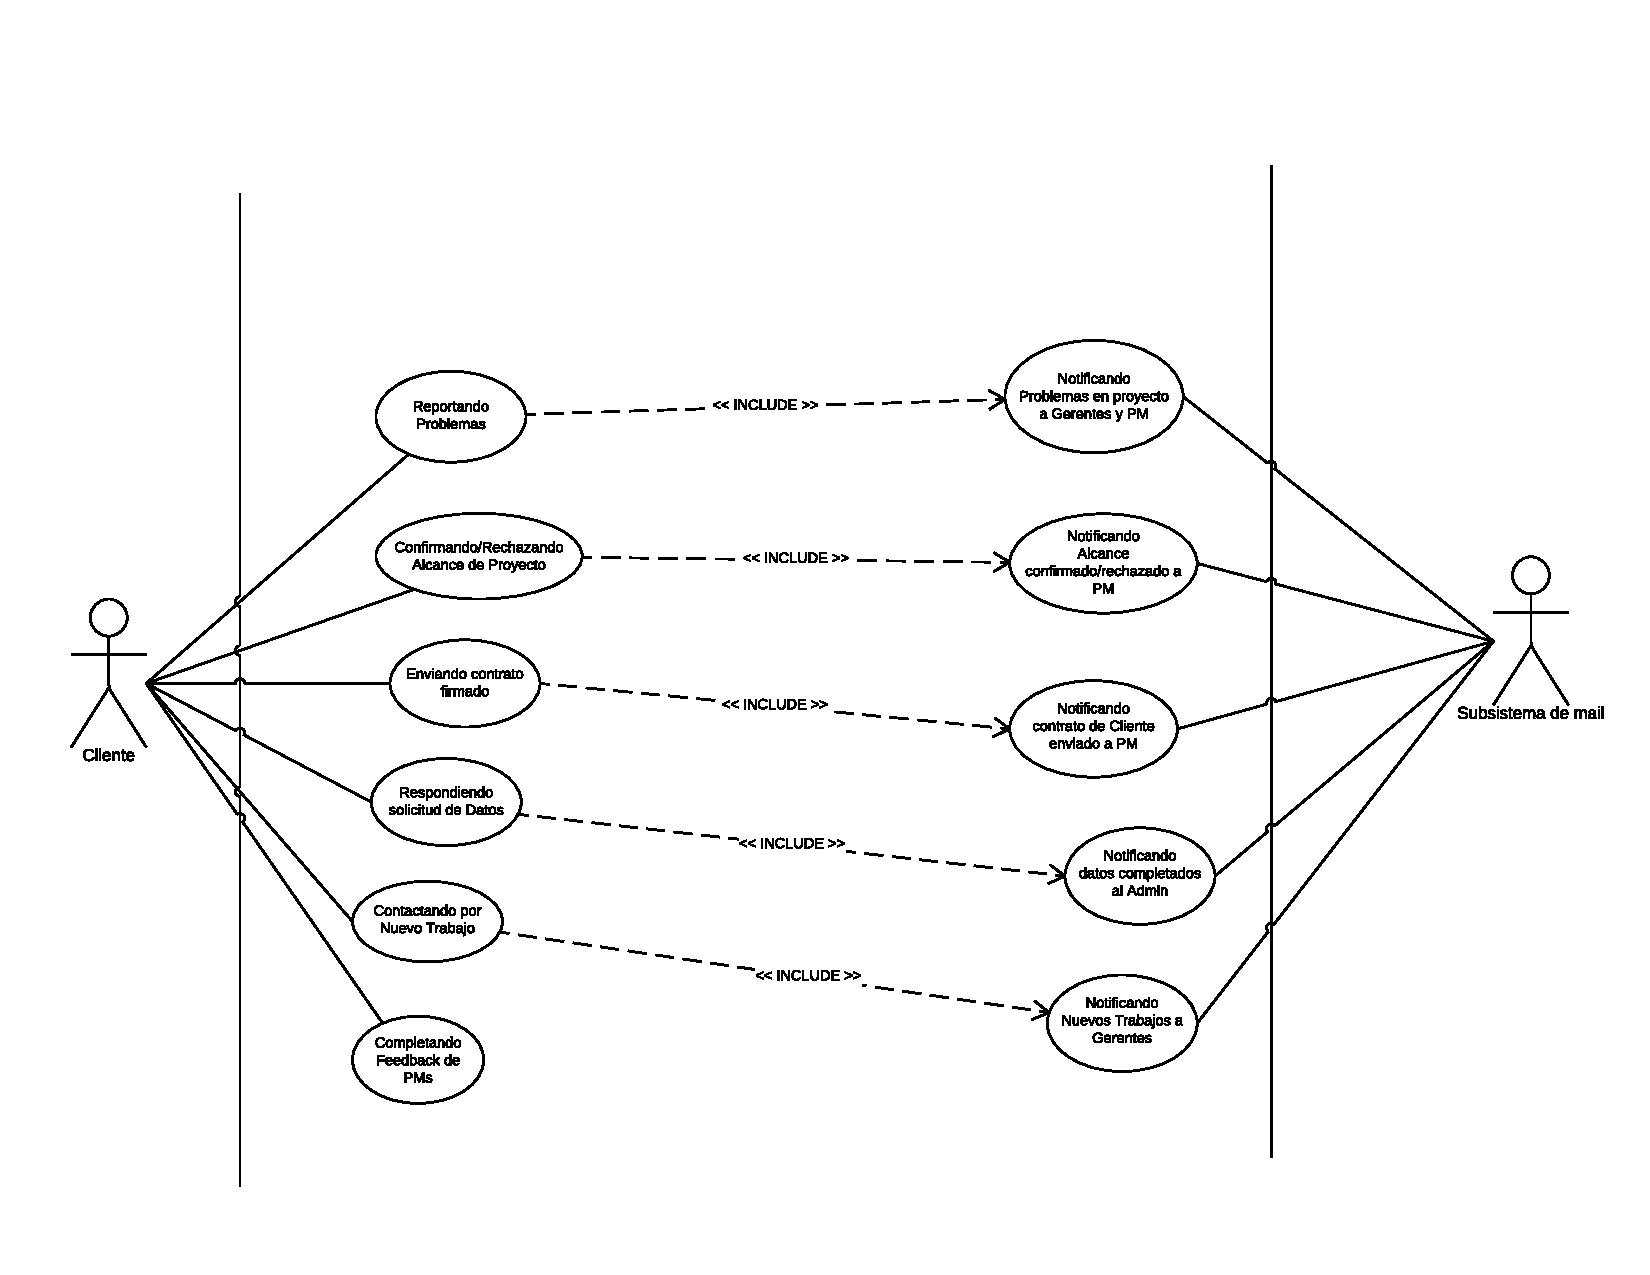
\includegraphics[width=\linewidth]{cu1.pdf}
\end{figure}
\begin{figure}[H]
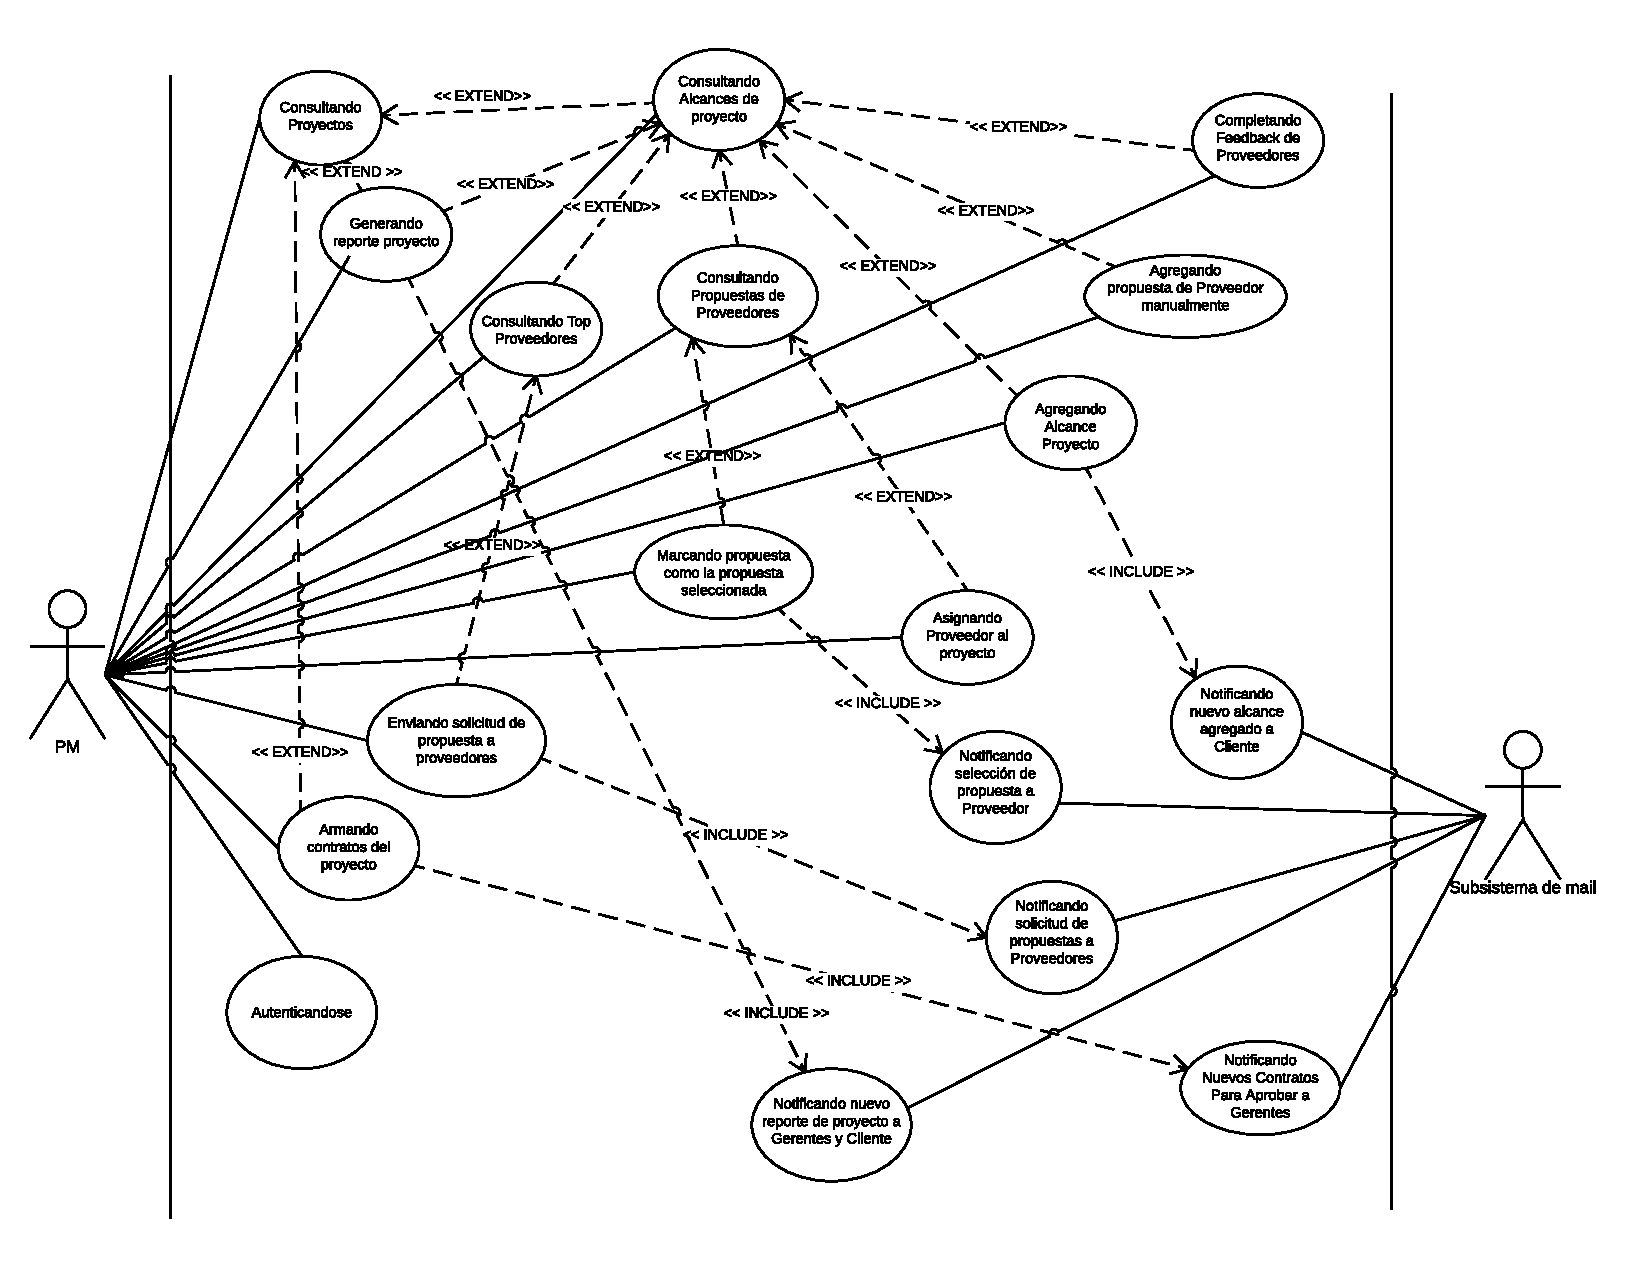
\includegraphics[width=\linewidth]{cu2.pdf}
\end{figure}
\begin{figure}[H]
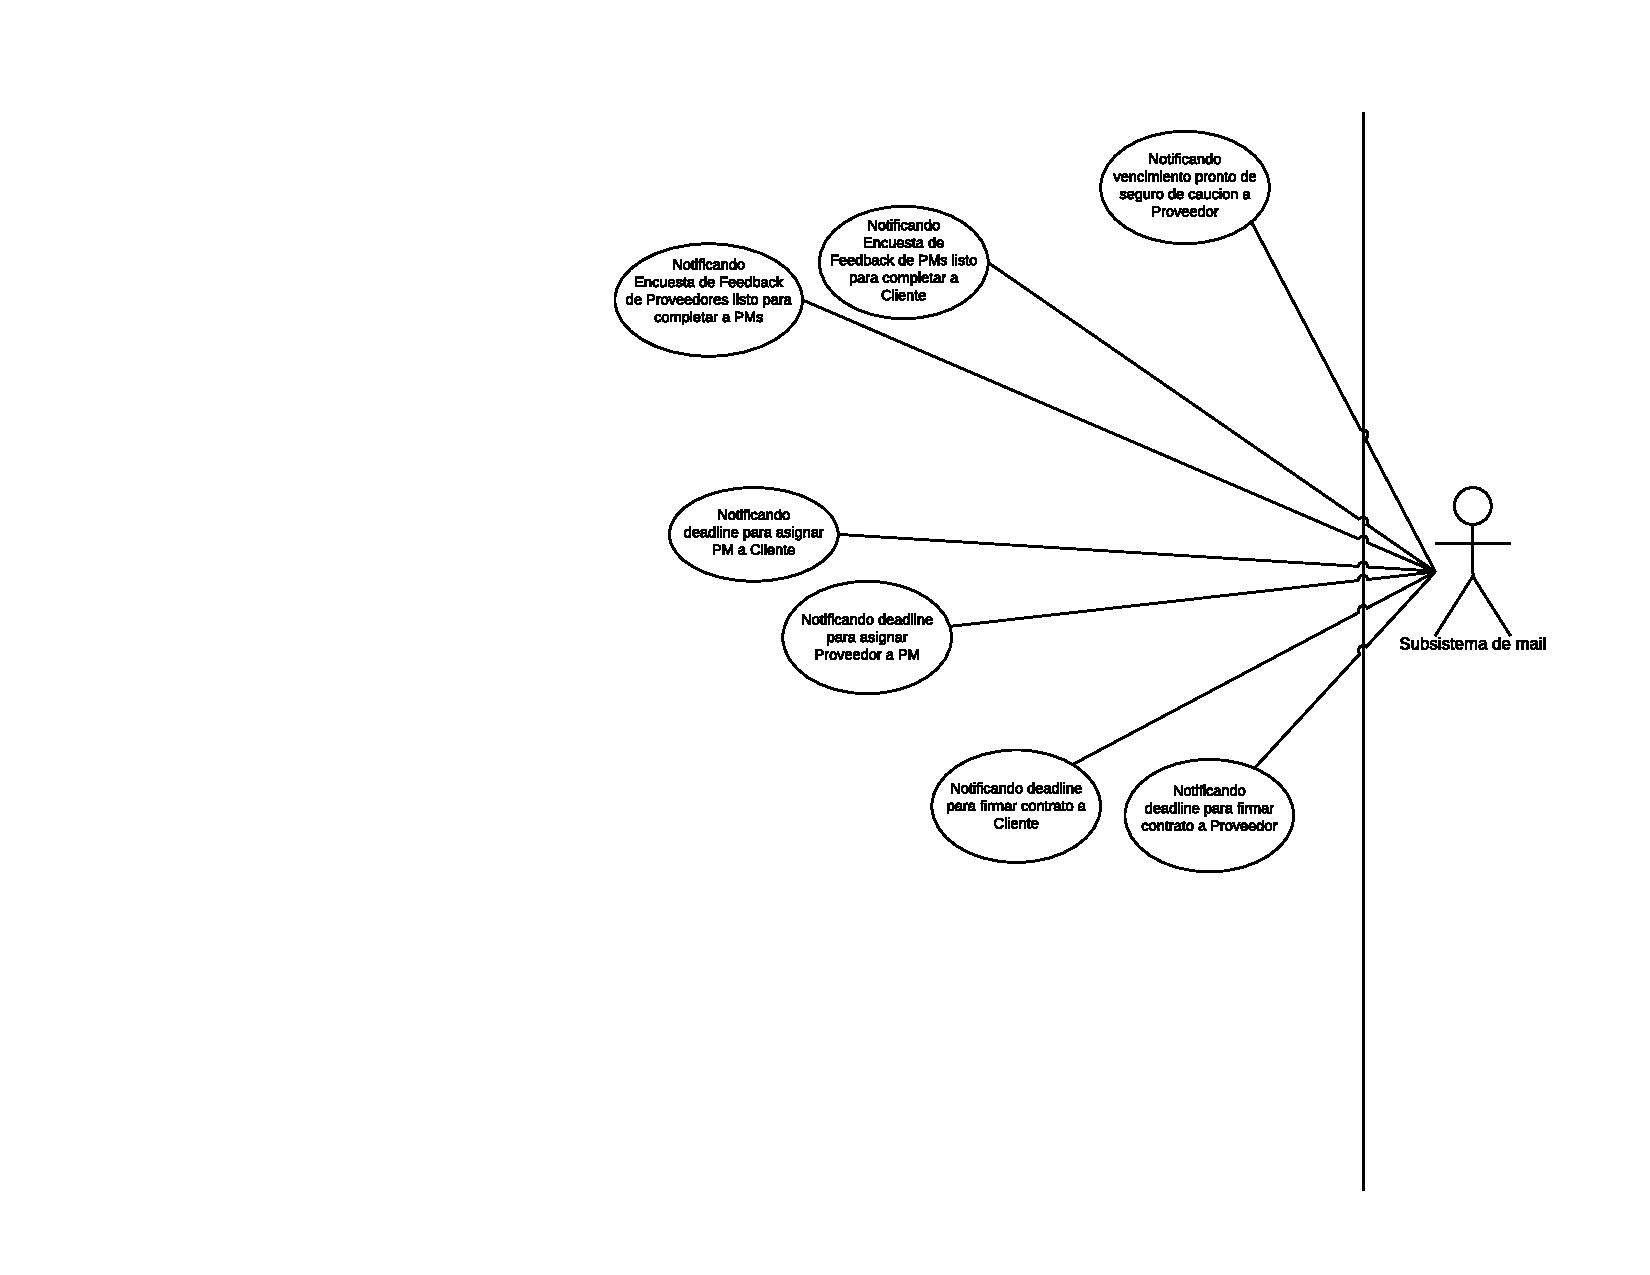
\includegraphics[width=\linewidth]{cu3.pdf}
\end{figure}
\begin{figure}[H]
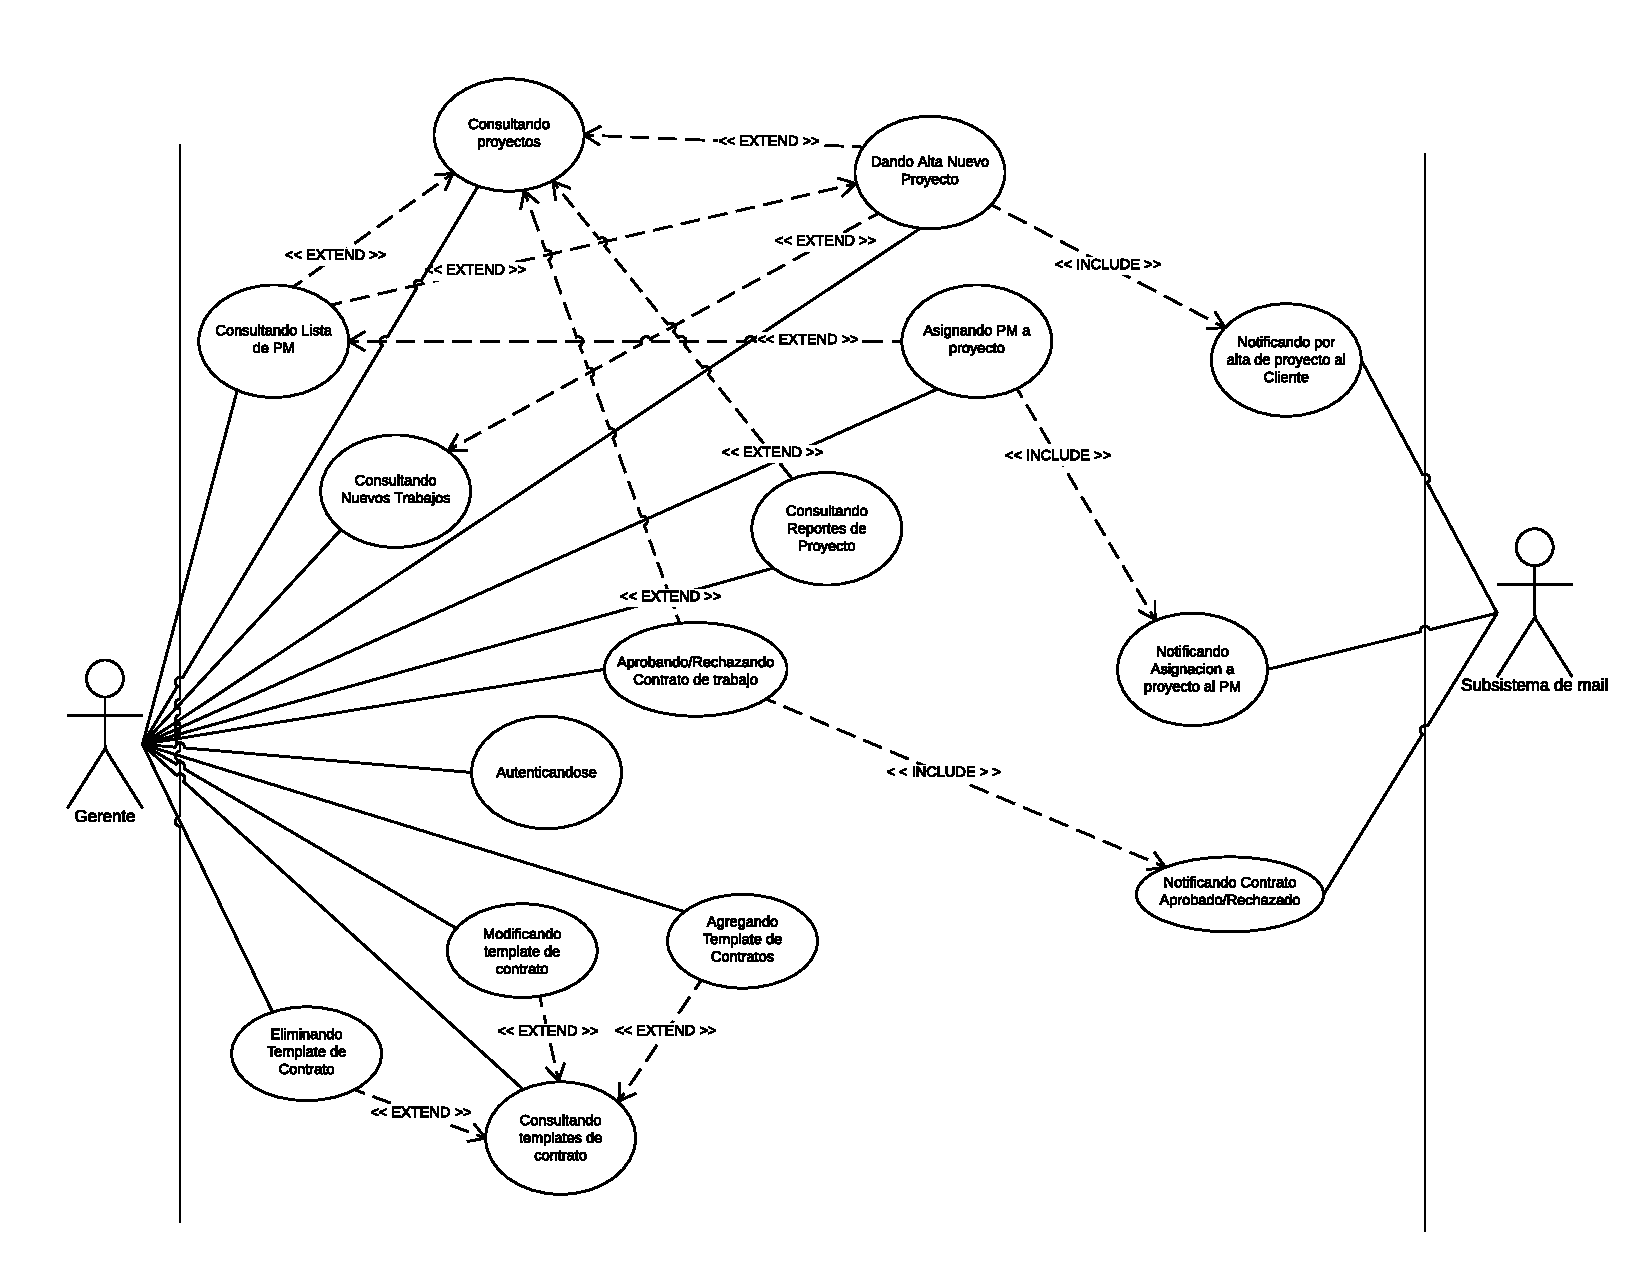
\includegraphics[width=\linewidth]{cu4.pdf}
\end{figure}
\begin{figure}[H]
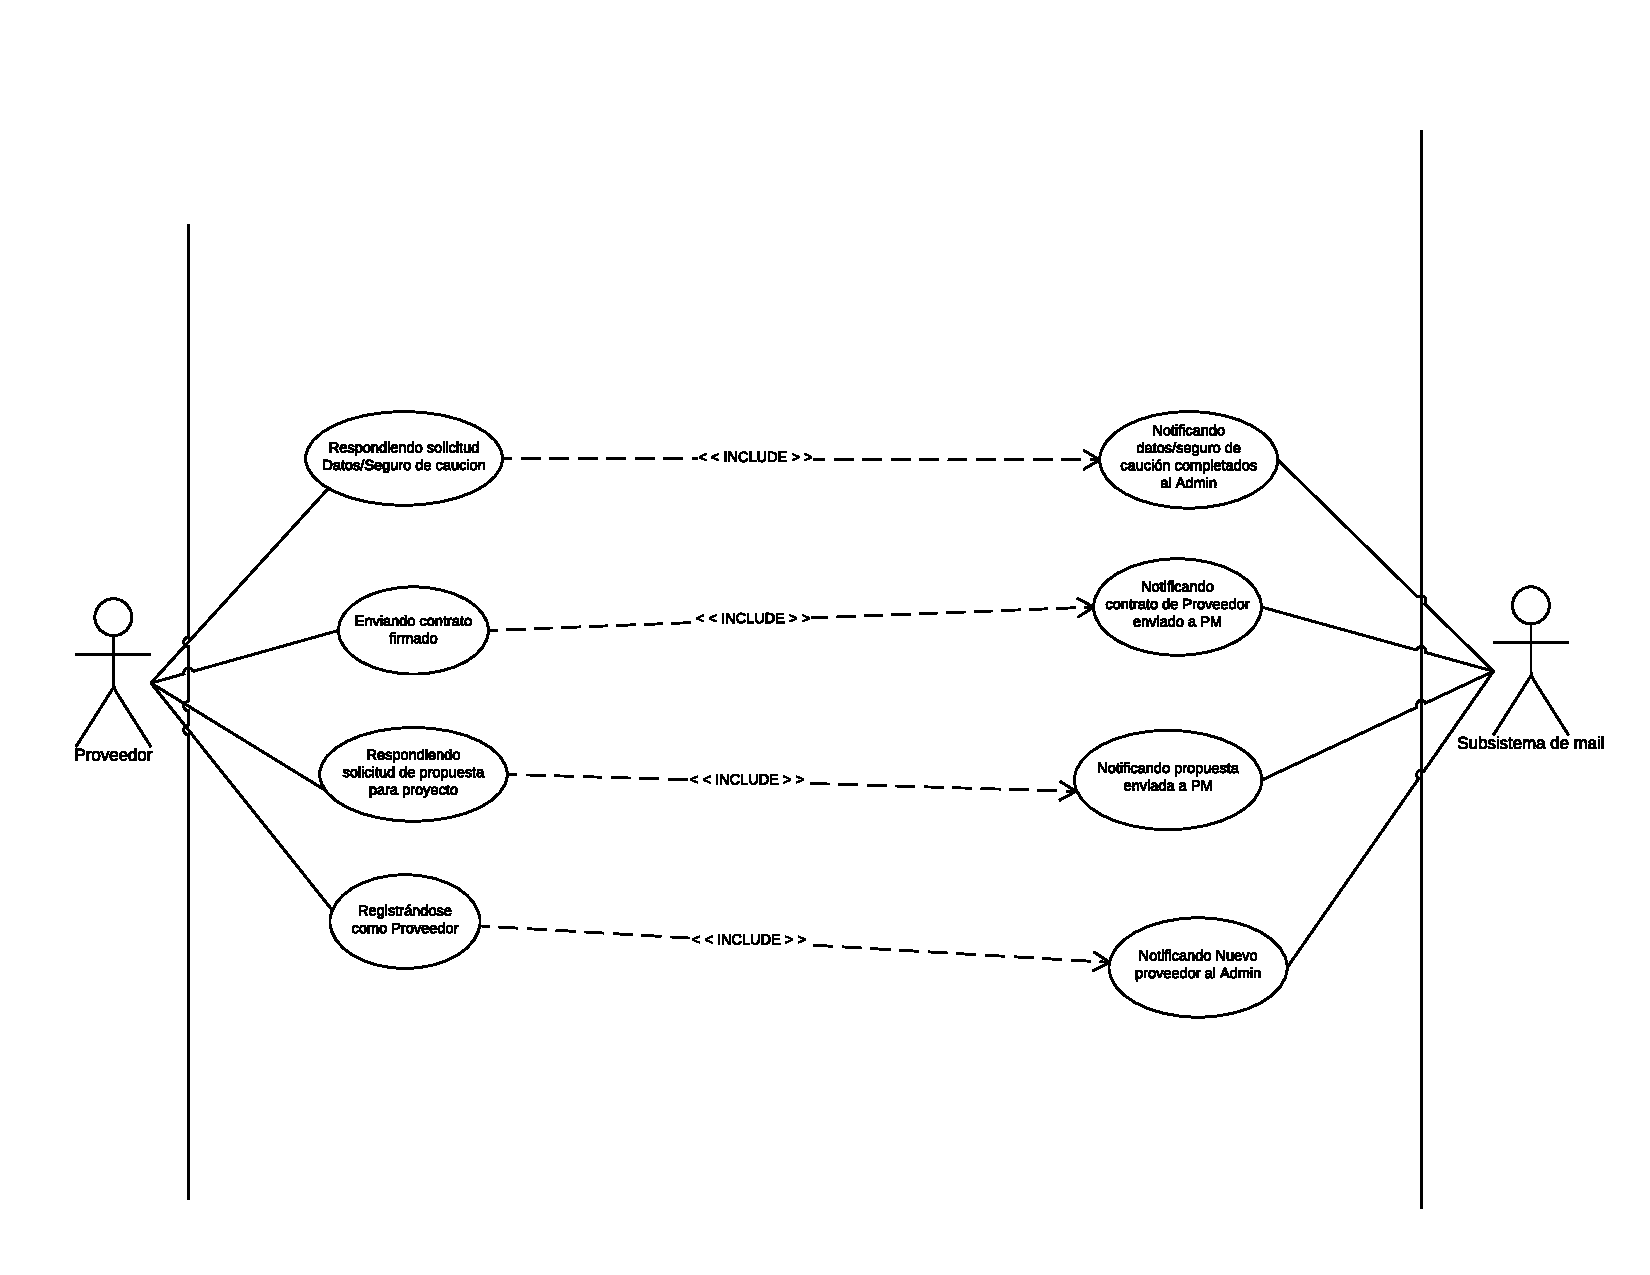
\includegraphics[width=\linewidth]{cu5.pdf}
\end{figure}
\begin{figure}[H]
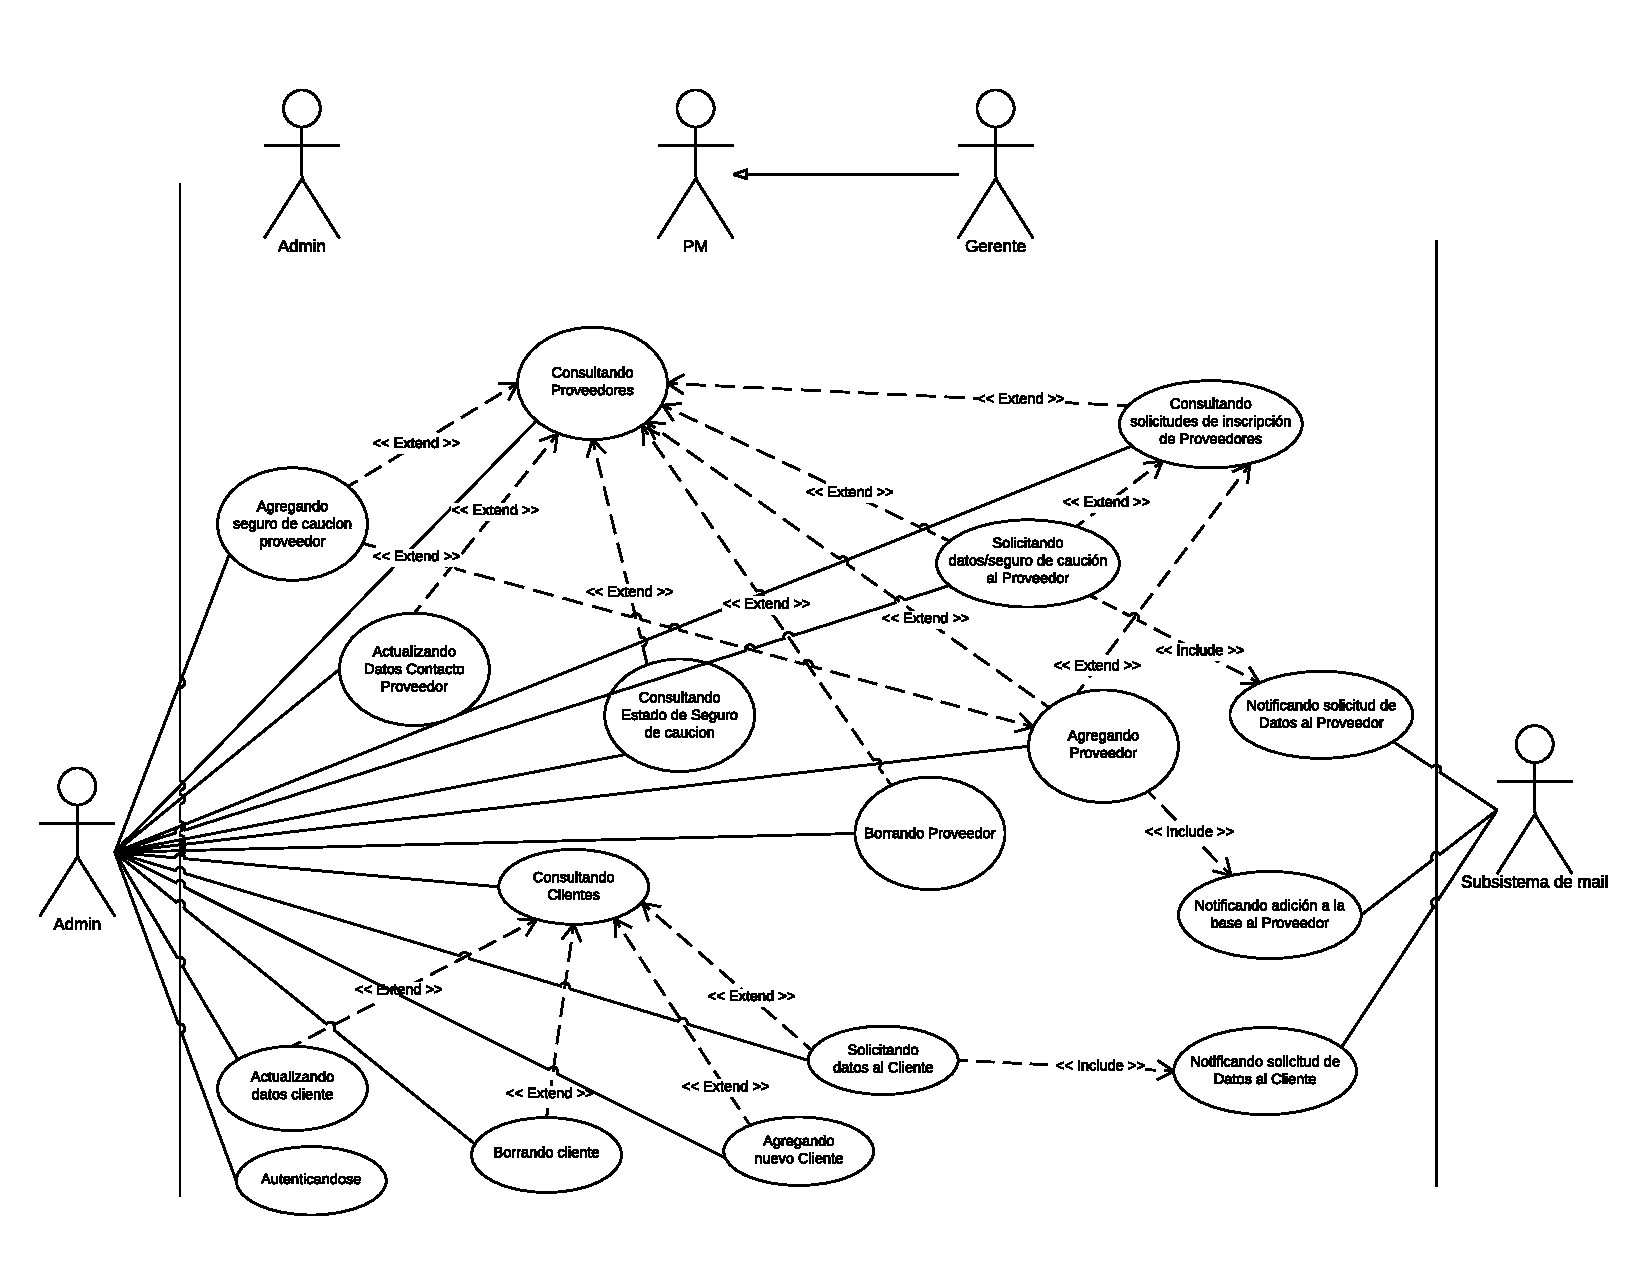
\includegraphics[width=\linewidth]{cu6.pdf}
\end{figure}

Para finalizar detallaremos los distintos casos de uso en los que ademas intentaremos ver cuales son los comportamientos alternativos que pueda tener nuestro sistema en las distintas sircunstancias.

% ADMIN
\begin{longtable}{| p{.60\textwidth} | p{.40\textwidth} |} 
    \hline
    \multicolumn{2}{|p{16cm}|}{
        \textbf{Caso de uso:} Consultando Proveedores \newline
        \textbf{Actor:} Administrador\newline
        \textbf{Pre:}  True\newline
        \textbf{Post:}El Administrador consulta el proveedor.
    }\\
    \hline
    1.El sistema le solicita que ingrese los filtros de busqueda  & 1.1.Sistema no  disponible por el momento.\newline 1.2Fin de C.U.\\
    \hline
    2.El Administrador Agrega los datos del provedor que esta buscando& \\
    \hline
    3.El Sistema encuentra el proveedor y muestra los datos & 3.1.El proveedor solicitado no se encuentra en el sistema \newline 3.2 Fin de C.U.  \\
    \hline
    4.El Administrador decide elimiar el proveedor. Extiende Caso de uso Eliminando Proveedor.& \\
    \hline
    5.El Administrador decide agregar el seguro de Caucion de proveedor. Extiende Caso de uso Agregando Seguro de Caucion.& \\
    \hline
    6.El Administrador decide consultar estado del seguro de Caucion de proveedor. Extiende Caso de uso Consultando estado de seguro de caucion.& \\
    \hline
    7.El Administrador decide consultar datos del proveedor. Extiende Caso de uso Consultando datos de proveedor.& \\
    \hline
    8.Fin de C.U.& \\
    \hline
\end{longtable}

\begin{longtable}{| p{.60\textwidth} | p{.40\textwidth} |} 
    \hline
    \multicolumn{2}{|p{16cm}|}{
        \textbf{Caso de uso:} Agregando Proveedor \newline
        \textbf{Actor:} Admin\newline
        \textbf{Pre:}  True\newline
        \textbf{Post:} El proveedor fue agregado al sistema
    }\\
    \hline
    1.El sistema le solicita que ingrese los datos del proveedor & 1.1.Sistema no  disponible por el momento.\newline 1.2Fin de C.U.\\
    \hline
    2.El Administrador Agrega los datos del provedor como son nombres, datos de contacto y datos relacionados al negocio &  \\
    \hline
    3.El Sistema valida los datos para ver si no se encuentra registrado & 3.1.El proveedor ya esta dado de alta \newline 3.2 Fin de C.U.  \\
    \hline
    4.El Sistema Pregunta si desea Agregar el seguro de caucion&\\
    \hline
    5.El Administrador Agrega Seguro de caucion, Extiende Caso de Uso Agregar seguro de Caucion. & 5.1 El Administrador decide agregarlo luego. Continua en paso 5 \\
    \hline
    6.Fin de C.U.& \\
    \hline
\end{longtable}

\begin{longtable}{| p{.60\textwidth} | p{.40\textwidth} |} 
    \hline
    \multicolumn{2}{|p{16cm}|}{
        \textbf{Caso de uso:} Borrando Proveedor \newline
        \textbf{Actor:} Administrador\newline
        \textbf{Pre:}  Autenticado como proveedor\newline
        \textbf{Post:} El proveedor fue eliminado del sistema
    }\\
    \hline
    1.El sistema  muetra las opciones para realizar con un proveedor & 1.1.Sistema no  disponible por el momento.\newline 1.2Fin de C.U.\\
    \hline
    2.El Administrador selecciona eliminar& \\
    \hline
    3.El Sistema lanza un mensaje consultando si desea eliminar el proveedor &  \\
    \hline
    4.El Administrador selecciona que SI desea eliminar el proveedor & 4.1.1 El Sistema nota que el proveedor sigue asignado a un proyecto en curso, muestra un mensaje por pantalla notificando este problema \newline 4.1.2 Fin Caso de Uso \newline 4.2.1 El usuario Selecciona que NO desea eliminar el proveedor \newline4.2.2 Fin de Caso de uso\\
    \hline
    5.El Sistema elimina el proveedor del sistema &  \\
    \hline
    6.Fin de C.U.& \\
    \hline
\end{longtable}
\begin{longtable}{|p{.60\textwidth}|p{.40\textwidth}|}
    \hline
    \multicolumn{2}{|p{16cm}|}{
        \textbf{Caso de uso:} Actualizando datos de Proveedor \newline
        \textbf{Actor:} Administrador\newline
        \textbf{Pre:true }  Autenticado como proveedor\newline
        \textbf{Post:} El Administrador actualiza los datos del Proveedor
    }\\
    \hline
    1.El sistema  muetra las opciones para realizar con un proveedor & 1.1.Sistema no  disponible por el momento.\newline 1.2Fin de C.U.\\
    \hline
    2.El Administrador selecciona Actualizar Datos Proveedor&   \\
    \hline
    3.El Sistema muestra todos los campos con los datos del proveedor para modificar y dos botones , uno para guardar y otro para cancelar&  \\
    \hline
    4.El Administrador Modifica los datos y toca salvar & 4.1.El Administrador toca cancelar \newline 4.2 Fin Caso de Uso \\
    \hline
    5.El Sistema guarda los cambios al proveedor &  \\
    \hline
    6.Fin de C.U.& \\
    \hline
\end{longtable}

\begin{longtable}{|p{.60\textwidth}|p{.40\textwidth}|}
    \hline
    \multicolumn{2}{|p{16cm}|}{
        \textbf{Caso de uso:} Consultando estado de seguro de caucion \newline
        \textbf{Actor:} Administrador\newline
        \textbf{Pre:true }  True\newline
        \textbf{Post:} El Administrador consulta estado del seguro de caucion
    }\\
    \hline
    1.El sistema  muetra las opciones para realizar con un proveedor & 1.1.Sistema no  disponible por el momento.\newline 1.2Fin de C.U.\\
    \hline
    2.El Administrador selecciona la opcion consultar estado de seguro de caucion&  \\
    \hline
    3.El Sistema muestra el estado de seguro de caucion&  \\
    \hline
    4.Fin de C.U.& \\
    \hline
\end{longtable}

\begin{longtable}{|p{.60\textwidth}|p{.40\textwidth}|}
    \hline
    \multicolumn{2}{|p{16cm}|}{
        \textbf{Caso de uso:} Agregando seguro de caucion\newline
        \textbf{Actor:} Administrador\newline
        \textbf{Pre:true }  Autenticado como proveedor\newline
        \textbf{Post:} El Administrador Agrega un nuevo seguro de caucion
    }\\
    \hline
    1.El sistema  muetra las opciones para realizar con un proveedor & 1.1.Sistema no  disponible por el momento.\newline 1.2Fin de C.U.\\
    \hline
    2.El Administrador selecciona la opcion agregar de seguro de caucion& \\
    \hline
    3.El Sistema muestra la opcion de ingreso de validez del seguro de caucion y el ingreso del archivo con el seguro de caucion&  \\
    \hline
    4.El Administrador ingresa la fecha de validez, agrega el archivo del escaneo del seguro de caucion y guarda los cambios&4.1 El administrador Apreta el boton cancelar \newline 4.2 Fin del Caso de uso \\
    \hline
    5.El Sistema verifica la fecha de validez y que no que no exista otro seguro de caucion & \\
    \hline
    6.El Sistema aprueba los datos ingresados y guarda los cambios &6.1 Los datos ingresados son incorrectos, o hay otro seguro de caucion en la misma fecha  \newline 6.2 vuelve al paso 4\\
    \hline
    7.Fin de C.U.& \\
    \hline
\end{longtable}

\begin{longtable}{|p{.60\textwidth}|p{.40\textwidth}|}
    \hline
    \multicolumn{2}{|p{16cm}|}{
        \textbf{Caso de uso:} Solicitando datos/seguro de caucion de proveedor\newline
        \textbf{Actor:} Administrador\newline
        \textbf{Pre:true }  Autenticado como proveedor\newline
        \textbf{Post:} El Administrador Agrega un nuevo seguro de caucion
    }\\
    \hline
    1.El sistema  muetra las opciones para realizar con un proveedor & 1.1.Sistema no  disponible por el momento.\newline 1.2Fin de C.U.\\
    \hline
    2.El Administrador selecciona la opcion agregar de seguro de caucion& \\
    \hline
    3.El Sistema muestra la opcion de ingreso de validez del seguro de caucion y el ingreso del archivo con el seguro de caucion&  \\
    \hline
    4.El Administrador ingresa la fecha de validez, agrega el archivo del escaneo del seguro de caucion y guarda los cambios&4.1 El administrador Apreta el boton cancelar \newline 4.2 Fin del Caso de uso \\
    \hline
    5.El Sistema verifica la fecha de validez y que no que no exista otro seguro de caucion & \\
    \hline
    6.El Sistema aprueba los datos ingresados y guarda los cambios &6.1 Los datos ingresados son incorrectos, o hay otro seguro de caucion en la misma fecha  \newline 6.2 vuelve al paso 4\\
    \hline
    7.Fin de C.U.& \\
    \hline
\end{longtable}


% cliente

\begin{longtable}{|p{.60\textwidth}|p{.40\textwidth}|}
    \hline
    \multicolumn{2}{|p{16cm}|}{
        \textbf{Caso de uso:} Contactando por nuevos trabajos\newline
        \textbf{Actor:} Cliente\newline
        \textbf{Pre:true }  True\newline
        \textbf{Post:} El Cliente deja el contacto para un nuevo trabajo en el sistema
    }\\
    \hline
    1.El sistema muestra las diferentes opciones para clientes & 1.1.Sistema no  disponible por el momento.\newline 1.2Fin de C.U.\\
    \hline
    2.El Cliente seleccion la opcion de contacto y completa los datos de contacto&2.1 El Cliente no ingresa datos de contacto\newline 2.2 Fin caso de uso   \\
    \hline
    3.El Sistema notifica nuevo proyecto. USA Caso de uso Notifica nuevo proyecto& \\
    \hline
    4.Fin de C.U.& \\
    \hline
\end{longtable}



\begin{longtable}{|p{.60\textwidth}|p{.40\textwidth}|}
    \hline
    \multicolumn{2}{|p{16cm}|}{
        \textbf{Caso de uso:} Notificando Encuesta para completar\newline
        \textbf{Actor:} Subsistema de Mail\newline
        \textbf{Pre:true }  True\newline
        \textbf{Post:} El Sistema envia un link para acceder a la encuesta para completar
    }\\
    \hline
    1.El sistema genera un cliente y se lo envia al subsistema de mail con los datos de envio & 1.1.Sistema no  disponible por el momento.\newline 1.2Fin de C.U.\\
    \hline
    2.El subsistema de mail genera un mail con remitente el que envio el sistema en la notificacion y le envia un mail con el link enviado adjuntado&   \\
    \hline
    3.Fin de C.U.& \\
    \hline
\end{longtable}


\begin{longtable}{|p{.60\textwidth}|p{.40\textwidth}|}
    \hline
    \multicolumn{2}{|p{16cm}|}{
        \textbf{Caso de uso:} Completando Feedback de PM\newline
        \textbf{Actor:} Cliente\newline
        \textbf{Pre: }Recibe notificacion para completar encuesta\newline
        \textbf{Post: }El Cliente Completo la encuesta
    }\\
    \hline
    1.El Usuario accede al link que recibe en el Mail y le abre una pagina web con la encuesta a completar & 1.1.El Usuario desestima el mail .\newline 1.2Fin de C.U.\\
    \hline
    2.El Usuario Completa las preguntas de la encuesta y agrega recomendaciones en caso de tenerlas&    \\
    \hline
    3.El Usuario Apreta el boton de Send y envia el formulario& \\
    \hline
    4.El Sistema Registra la nueva encuesta&\\
    \hline
    5.Fin del C.U&\\
    \hline
\end{longtable}
% PM

\begin{longtable}{|p{.60\textwidth}|p{.40\textwidth}|}
    \hline
    \multicolumn{2}{|p{16cm}|}{
        \textbf{Caso de uso:}Consultando Proyectos\newline
        \textbf{Actor:} PM\newline
        \textbf{Pre: }El PM esta logueado en el sistema\newline
        \textbf{Post:} El PM ve todos los proyectos registrados en el sistema
    }\\
    \hline
    1.El PM ingresa al sistema& \\
    \hline
    2.El sistema muestra todas las opciones de interaccion disponible&  \\
    \hline
    3.El PM selecciona buscar proyectos& \\
    \hline
    4.El sistema muestra todos los proyectos disponibles&4.1 El PM filtra la lista de proyectos por id o por cliente\\
    \hline
    5.Fin del C.U&\\
    \hline
\end{longtable}

\begin{longtable}{|p{.60\textwidth}|p{.40\textwidth}|}
    \hline
    \multicolumn{2}{|p{16cm}|}{
        \textbf{Caso de uso:}Consultando alcance de Proyectos\newline
        \textbf{Actor:} PM\newline
        \textbf{Pre: }El PM busco un proyecto\newline
        \textbf{Post:} El PM Puede ve los alcances de un proyecto
    }\\
    \hline
    1.El sistema muestra las opciones del proyecto& \\
    \hline
    2.El PM selecciona ver los alcances del proyecto&  \\
    \hline
    3.El sistema muestra los alcances del proyectos& \\
    \hline
    4.Fin del C.U&\\
    \hline
\end{longtable}

\begin{longtable}{|p{.60\textwidth}|p{.40\textwidth}|}
    \hline
    \multicolumn{2}{|p{16cm}|}{
        \textbf{Caso de uso:}Consultando TOP de proveedores\newline
        \textbf{Actor:} PM\newline
        \textbf{Pre: }El PM se loguea en el sistema\newline
        \textbf{Post:} El PM obtiene una lista de proveedores ordenados segun los filtros seleccionados
    }\\
    \hline
    1.El sistema muestra los filtros de busqueda& \\
    \hline
    2.El PM completa los filtros de busqueda&  \\
    \hline
    3.El sistema muestra los resultados basado en los filtros de busqueda ordenados por algun criterio seleccionado& \\
    \hline
    4.Fin del C.U&\\
    \hline
\end{longtable}


\begin{longtable}{|p{.60\textwidth}|p{.40\textwidth}|}
    \hline
    \multicolumn{2}{|p{16cm}|}{
        \textbf{Caso de uso:}Consultando propuestas de los proveedores\newline
        \textbf{Actor:} PM\newline
        \textbf{Pre: }El PM busco un proyecto\newline
        \textbf{Post:} El PM obtiene una lista de las propuestas presentadas por los proveedores
    }\\
    \hline
    1.El sistema muestra las distintas opciones en la pantalla de detalle de proyecto& \\
    \hline
    2.El PM selecciona la opcion de ver propuestas presentadas&\\
    \hline
    3.El sistema muestra las propuestas presentadas por los distintos proveedores & \\
    \hline
    4.El PM selecciona una propuesta  &\\
    \hline
    5.El sistema muestra el detalle de la propeusta seleccionada&\\
    \hline
    6.Fin del C.U&\\
    \hline
\end{longtable}

\begin{longtable}{|p{.60\textwidth}|p{.40\textwidth}|}
    \hline
    \multicolumn{2}{|p{16cm}|}{
        \textbf{Caso de uso:}Marcando una propuesta como seleccionada\newline
        \textbf{Actor:} PM\newline
        \textbf{Pre: }El PM busco las propuestas asociadas a un proyecto\newline
        \textbf{Post:} El PM selecciona una de las propeustas para el proyecto seleccionado
    }\\
    \hline
    1.El sistema muestra las propeustas para el proyecto seleccionado& \\
    \hline
    2.El PM selecciona una propuesta para el proyecto y guarda los cambios&\\
    \hline
    3.El sistema envia una notificacion al proeedor.USA Notificando seleccion de propuesta a proveedor& \\
    \hline
    4.Fin del C.U&\\
    \hline
\end{longtable}

\begin{longtable}{|p{.60\textwidth}|p{.40\textwidth}|}
    \hline
    \multicolumn{2}{|p{16cm}|}{
        \textbf{Caso de uso:}Generando reporte de proyecto\newline
        \textbf{Actor:} PM\newline
        \textbf{Pre: }El PM busco un proyecto\newline
        \textbf{Post:} El PM agrega un detalle de los avances en el proyecto
    }\\
    \hline
    1.El sistema muestra las distintas opciones en la pantalla de detalle de proyecto& \\
    \hline
    2.El PM selecciona la opcion de agregar reporte &\\
    \hline
    3.El sistema muestra las un formulario para completar& \\
    \hline
    4.El PM completa un formulario con los avances del proyecto y guarda el reporte&\\
    \hline
    5.El sistema guarda el formulario&\\
    \hline
    6.Fin del C.U&\\
    \hline
\end{longtable}


\begin{longtable}{|p{.60\textwidth}|p{.40\textwidth}|}
    \hline
    \multicolumn{2}{|p{16cm}|}{
        \textbf{Caso de uso:}Enviando solicitud de propeusta a proveedores\newline
        \textbf{Actor:} PM\newline
        \textbf{Pre: }El PM busco el TOP de proveedores\newline
        \textbf{Post:} El PM envia la soliicitud de propuestas a los mejores proveedores
    }\\
    \hline
    1.El sistema muestra la lista de TOP de proveedores & \\
    \hline
    2.El PM selecciona varios proveedores y selecciona la opcion de enviar solicitud de propuesta& \\
    \hline
    3.El sistema envia la notificacion.USA Notificando solicitud de porpuestas a proveedores& \\
    \hline
    4.Fin del C.U&\\
    \hline
\end{longtable}

% GERENTE
\begin{longtable}{|p{.60\textwidth}|p{.40\textwidth}|}
    \hline
    \multicolumn{2}{|p{16cm}|}{
        \textbf{Caso de uso:}Asignando PM Al Proyecto\newline
        \textbf{Actor:} Gerente\newline
        \textbf{Pre: }true\newline
        \textbf{Post:} Un PM es asignado al proyecto
    }\\
    \hline
    1.El Gerente ingresa al sistema & \\
    \hline
    2.El Gerente Consulta los proyectos nuevos en el sistema USA Consultando Nuevos Trabajos&    \\
    \hline
    3.El Gerente Consulta los mejores PM para el proyecto dado USA Consutlando TOP Proveedores& \\
    \hline
    4.El Gerente Asigna el mejor PM Al Proyecto&\\
    \hline
    5.Fin del C.U&\\
    \hline
\end{longtable}


\begin{longtable}{|p{.60\textwidth}|p{.40\textwidth}|}
    \hline
    \multicolumn{2}{|p{16cm}|}{
        \textbf{Caso de uso:}Consultando Top Proveedores\newline
        \textbf{Actor:} Gerente\newline
        \textbf{Pre: }true\newline
        \textbf{Post:}  El Gerente obtiene una lista con los mejores provedores ordenados
    }\\
    \hline
    1.El Gerente ingresa al sistema & \\
    \hline
    2.El Gerente Consulta Los proveedores seleccionando filtros de busqueda&    \\
    \hline
    3.El Sistema le devuelve al gerente una lista de los mejores proveedores para sus filtros de busqueda& \\
    \hline
    4.Fin del C.U&\\
    \hline
\end{longtable}


\begin{longtable}{|p{.60\textwidth}|p{.40\textwidth}|}
    \hline
    \multicolumn{2}{|p{16cm}|}{
        \textbf{Caso de uso:}Consultando Status de proyecto\newline
        \textbf{Actor:} Gerente\newline
        \textbf{Pre: }true\newline
        \textbf{Post:}  El Gerente Consulta el estado de un proyecto
    }\\
    \hline
    1.El Gerente ingresa al sistema & \\
    \hline
    2.El Gerente Busca un proyecto segun ciertos filtros&    \\
    \hline
    3.El Sistema le devuelve una lista de proyectos& \\
    \hline
    4.El Gerente Selecciona un proyecto y presiona el boton de obtener estado de proyecto&\\
    \hline
    5.El Sistema Devuelve el estado del proyecto seleccionado &\\
    \hline
    6.Fin del C.U.&\\
    \hline
\end{longtable}


\begin{longtable}{|p{.60\textwidth}|p{.40\textwidth}|}
    \hline
    \multicolumn{2}{|p{16cm}|}{
        \textbf{Caso de uso:}Consultando top proveedores \newline
        \textbf{Actor:} PM \newline
        \textbf{Pre: }true\newline
        \textbf{Post:}  El PM Obtiene una lista de los mejores proveedores para el proyecto
    }\\
    \hline
    1.El PM ingresa los datos del proyecto y selecciona la opcion obtener mejores proveedores& \\
    \hline
    2.El sistema devuelve una lista de los mejores proveedores que se ajustan al proyecto&    \\
    \hline
    3.Fin del C.U.&\\
    \hline
\end{longtable}
